\documentclass[a4paper,11pt]{article}

\usepackage{fullpage}
\usepackage[utf8]{inputenc}
\usepackage{t1enc}
\usepackage[spanish]{babel}
\usepackage[pdftex,usenames,dvipsnames]{color}
\usepackage[pdftex]{graphicx}
\usepackage{enumerate}
\usepackage{url}
\usepackage{amsmath}
\usepackage{amsfonts}
\usepackage{amssymb}
\usepackage{comment}
\usepackage[table]{xcolor}
\usepackage[small,bf]{caption}
\usepackage{float}
\usepackage{subfig}
\usepackage{bm}
\usepackage{fancyhdr}
\usepackage{times}
\usepackage{titlesec}
\usepackage{csquotes}
\usepackage[backend=bibtex,sorting=none]{biblatex}
\usepackage{titling}
% \usepackage{algorithmicx}
\usepackage{algpseudocode}
\usepackage{algorithm}
\usepackage{letltxmacro}
\usepackage[margin=1cm]{caption}
\usepackage{chngcntr}

%%%%% BEGIN ALGPSEUDOCODE STUFF %%%%%%
\algdef{SxnE}[FOREACH]{ForEach}{EndFor}[1]{\algorithmicfor\ #1\ \algorithmicdo}
% LEAVES BLANK LINE AT END \algblockdefx[FOREACH]{ForEach}{EndFor}{\textbf{for each }}{}
\algdef{SxnE}[FOR]{For}{EndFor}[1]{\algorithmicfor\ #1\ \algorithmicdo}
\algdef{SxnE}[WHILE]{While}{EndWhile}[1]{\algorithmicwhile\ #1\ \algorithmicdo}
\algdef{SxnE}[IF]{If}{EndIf}[1]{\algorithmicif\ #1\ \algorithmicthen}
\algdef{cxnE}{IF}{Else}{EndIf}

\renewcommand{\algorithmicrequire}{\textbf{Input:}}
\renewcommand{\algorithmicensure}{\textbf{Output:}}
\algnewcommand\algorithmicauxiliary{\textbf{Auxiliary:}}
\algnewcommand\Auxiliary{\item[\algorithmicauxiliary]}

\DefineBibliographyStrings{spanish}{andothers = {et\addabbrvspace al\adddot}}
\renewbibmacro{in:}{}

\floatname{algorithm}{Algoritmo}

\DeclareMathOperator*{\argmin}{arg\,min}
\addbibresource{references}
\DeclareFieldFormat[inbook]{citetitle}{#1}

\newcommand{\norm}[1]{\left\lVert#1\right\rVert}

% \titleformat{\section}{\small\center\bfseries}{\thesection.}{0.5em}{\normalsize\uppercase}
% \titleformat{\subsection}{\small\center\bfseries}{}{0.5em}{\small\uppercase}

\def\customabstract{\vspace{.5em}
    {\small\center{\textbf{RESUMEN}} \\[0.5em] \relax%
    }}
\def\endkeywords{\par}

\def\keywords{\vspace{.5em}
    {\textit{Palabras clave: }
    }}
\def\endkeywords{\par}

% TITLE Configuration
\setlength{\droptitle}{-30pt}
\pretitle{\begin{center}\Huge\begin{rmfamily}}
\posttitle{\par\end{rmfamily}\end{center}\vskip 0.5em}
\preauthor{\begin{center}
        \large \lineskip 0.5em%
\begin{tabular}[t]{c}}
\postauthor{\end{tabular}\normalsize
    \\[1em] Instituto Tecnológico de Buenos Aires
\par\end{center}}
\predate{\begin{center}\small}
\postdate{\par\end{center}}

% Headers
\addtolength{\voffset}{-40pt}
\addtolength{\textheight}{80pt}
\renewcommand{\headrulewidth}{0pt}
\fancyhead{}
\fancyfoot{}
\lhead{\small } % No publicado
\rhead{\small \thepage}
\cfoot{\small Copyright \copyright 2013 ITBA}

% Next 4 lines allow for parts with independet sections counters
% and correct referencing between parts

\counterwithin*{section}{part}

\makeatletter

\def\p@section{\thepart.}
\def\p@subsection{\thepart.}
\def\p@subsubsection{\thepart.}

\makeatother

% Metadata
\title{Problemas para el Análisis Automático en Tiempo Real de Jugadas en Partidos de Futbol}
\date{20 de Septiembre de 2013}
\author{Civile, Juan Pablo \and Crespo, Álvaro \and Ordano, Esteban }


\begin{document}

\customabstract{
Las técnicas de seguimiento de objetos en videos tienen numerosas aplicaciones
en las actividades cotidianas. En el ámbito deportivo pueden ser útiles para
soportar (o hasta reemplazar) las decisiones de los jueces o árbitros del
juego, permitir a los deportistas mejorar su juego mediante el análisis de sus
movimientos, otorgar estadísticas y métricas a los fanáticos del deporte, entre
otras aplicaciones.

Se analiza en la primer parte de este trabajo el estado del arte respecto a
técnicas aplicables al problema de seguimiento de múltiples jugadores de fútbol
mediante el uso de una o varias cámaras de video, así como las bases teóricas
para estos métodos, características, limitaciones de cada uno, y la
factibilidad de conocer el estado del juego completo en cada instante de
tiempo.

Se plantea el uso de una de estas técnicas, \textit{contornos activos}, para
el seguimiento en tiempo real de los jugadores en base a una filmación
con una cámara fija abarcando todo el campo de juego. Se plantean mejoras
al algoritmo específicas a los fines del seguimiento de jugadores de fútbol.
}

\section{Introducción}

(Sacar pedazos de informe y de state-of-the-art)

\newpage

\part{Estado del arte}

\documentclass[a4paper,10pt]{article}

\usepackage[utf8]{inputenc}
\usepackage{t1enc}
\usepackage[spanish]{babel}
\usepackage[pdftex,usenames,dvipsnames]{color}
\usepackage[pdftex]{graphicx}
\usepackage{enumerate}
\usepackage{url}
\usepackage{amsmath}
\usepackage{amsfonts}
\usepackage{amssymb}
\usepackage[table]{xcolor}
\usepackage[small,bf]{caption}
\usepackage{float}
\usepackage{subfig}
\usepackage{bm}
\usepackage{fancyhdr}
\usepackage{times}
\usepackage{titlesec}
\usepackage{csquotes}
\usepackage[backend=bibtex]{biblatex}
\usepackage{titling}

\DeclareMathOperator*{\argmin}{arg\,min}
\addbibresource{references}
\DeclareFieldFormat[inbook]{citetitle}{#1}

\titleformat{\section}{\small\center\bfseries}{\thesection.}{0.5em}{\normalsize\uppercase}
\titleformat{\subsection}{\small\center\bfseries}{}{0.5em}{\small\uppercase}

\def\customabstract{\vspace{.5em}
    {\small\center{\textbf{RESUMEN}} \\[0.5em] \relax%
    }}
\def\endkeywords{\par}

\def\keywords{\vspace{.5em}
    {\textit{Palabras clave: } 
    }}
\def\endkeywords{\par}

% TITLE Configuration
\setlength{\droptitle}{-30pt}
\pretitle{\begin{center}\Huge\begin{rmfamily}}
\posttitle{\par\end{rmfamily}\end{center}\vskip 0.5em}
\preauthor{\begin{center}
        \large \lineskip 0.5em%
\begin{tabular}[t]{c}}
\postauthor{\end{tabular}\normalsize 
    \\[1em] Estudiantes del Instituto Tecnológico de Buenos Aires
\par\end{center}}
\predate{\begin{center}\small}
\postdate{\par\end{center}}

% Headers
\addtolength{\voffset}{-40pt}
\addtolength{\textheight}{80pt}
\renewcommand{\headrulewidth}{0pt}
\fancyhead{}
\fancyfoot{}
\lhead{\small No publicado}
\rhead{\small \thepage}
\cfoot{\small Copyright \copyright 2013 ITBA}

% Metadata
\title{}
\date{20 de Septiembre de 2013}
\author{Civile, Juan Pablo \and Crespo, Álvaro \and Ordano, Esteban }

\begin{document}

\pagestyle{fancy}
\maketitle
\thispagestyle{fancy}

\begin{customabstract}
\textbf{
}
\end{customabstract}

\begin{keywords}
\end{keywords}

\newpage

\part*{Estado del Arte}

% Describir la organizacion de esta seccion

\section{Una camara}

Conocemos 3 familias de algoritmos de tracking en video utilizando una sola camara.
Estas son \textit{Linear Predictors}, \textit{Local learning} y \textit{Graph based}.
Pasamos a describir las tecnicas usadas por estos.

\subsection{Linear predictors}

\textit{Linear Predictor} se refiere a crear una relacion lineal \[ Ax = b \] donde $A$ es un predictor, $x$ un valor medido y $b$ otro segundo valor relacionado a $x$ de alguna manera.
En \cite{alp, original-linear-predictors} los autores utilizan predictores que relacionan muestras tomadas de la imagen con el cambio de posicion del objeto.
Para obtener la relacion $A$ se utiliza un paso inicial de entrenamiento.
Se parte de una posicion conocida y se hacen multiples mutaciones obteniendo $N$ cambios de posiciones $b_i$ y sus correspondientes muestras $x_i$.
Luego se define $X = (x_1, \dots, x_N)$ y $B = (b_1, \dots, b_N)$ y se resuelve $AX = B$.

Una vez calculada $A$, en cada cuadro se toman muestras de la imagen usando la ultima posicion conocida del objeto.
Usando estas muestras se calcula el cambio de posicion del objeto mediante $Ax$.
Para mejorar la efectividad de los algoritmos, se calculan varios predictores y se disponen en capas.
Cada capa se construye para buscar cambios de posicion cada vez mas pequeños.
Es decir, la primer capa busca cambios bruscos y la ultima pequeños cambios.

\citeauthor*{alp} introducen varias tecnicas para hacer mas robusto el algoritmo.
Primero calculan la relacion $A$ de forma tal que puede ser facilmente actualizada para soportar cambios en el objeto.
Esto permite detectar oclusiones parciales y cambiar el predictor para que no busque las partes ocultas del objeto.
Una vez que las partes ocultas del objeto entran en el campo visual de vuelta, se vuelve a agregar las partes del predictor que se quitaron previamente.
Esta tecnica ademas permite reentrenar la relacion $A$ con poco costo computacional.
Luego, para soportar cambios de iluminacion en la imagen siempre ajustan las muestras tomadas a una distribucion normal.

\subsection{Local learning}
% Local learning

El aprendizaje local, o \textit{local learning}, puede resolver razonablemente el problema del seguimiento de objetos en secuencias de imágenes, lo
que ha sido un tema de investigación en el área del aprendizaje automático \cite{local-learning-machine-learnin} y usado principalmente en la clasificación 
de imágenes, recuperación y reconocimiento de objetos. A diferencia del aprendizaje global, \textit{global learning}, que entrena un modelo global basado en 
todos los datos de entrenamiento, local learning considera varios modelos locales, cada uno extraído de solamente un subconjunto de los datos de entrenamiento.
Este tipo de enfoque enfatiza la idea de que un modelo local puede caracterizar mejor las propiedades intrínsecas y discriminativas de su correspondiente 
subconjunto de datos, que un modelo global para el conjunto completo de datos. De esto se desprende que utilizar múltiples modelos locales puede ofrecer 
mejores resultados cuando los datos están distribuidos de manera complicadao o poco clara.\\
Si bien se puede pensar al seguimiento de objetos como una tarea de clasificación binaria 
que apunta a separar el objeto del resto de la imagen o fondo, en realidad, el principal
problema reside en relacionar las apariciones del objeto entre 2 cuadros, \textit{frames},
consecutivos. Es por esto que la métrica de distancia para determinar el grado de 
relación entre los puntos característicos del objeto adquiere muchísima importancia.
Una simple medida de distancia como la distancia Euclideana puede llevar a algoritmos
de tracking inestables a la hora de diferenciar el objeto del fondo de la imagen. Por
lo tano, es necesario diseñar una medida de distancia eficiente y discriminativa. Esta 
es la idea princial que proponen Li y Lu \cite{local-learning}.\\
La función de distancia que usan es una combinación lineal de distancias elementales, 
como se presenta en \cite{malisiewicz-cvpr08}. Definen a la función de distancia de un 
ejemplar (punto característico) $e$, $D_{e}$ como:

\begin{equation}
    \label{eq:distance-exemplar}
    D_{e}(z) = w_{e} \cdot d_{ez}
\end{equation}

donde $w_{e}$ es el vector de pesos de $e$, y $d_{ez}$ es el vector de distancia 
n-dimensional entre $e$ y $z$, cuya n-ésima componente es la distancia $L_{2}$ 
entre la característica n-ésima de $e$ y $z$.\\
Cada ejemplar está también asociado con un vector binario $B_{e}$, cuyos elementos 
no nulos implican que los ejemplares correspondientes son similares a $e$. La 
longitud de $B_{e}$ es igual al número de ejemplares con el mismo rótulo de $e$.
Asumiendo que el aprendizaje de cada una de las funciones de distancia es 
independiente del resto, se puede aprender $w_{e}$ y $B_{e}$, en un problema 
de aprendizaje formulado de la siguiente manera:

\begin{equation}
    \label{eq:learning-problem}
    f_{1}(w,B) = \sum_{i \in C} B_{i}L(-w \cdot d_{i}) + \sum_{i\notin C}L(w \cdot d_{i})
\end{equation}
\begin{equation}
    {w^{*}, B^{*} = \argmin_{w,b} f_{1} (w,b) }
\end{equation}
\begin{equation}
   w \geq 0, B_{i} \in {0,1}, \sum_{i} B_{i} = M
\end{equation}

El conjunto $C$ es el conjunto de todos los ejemplares con el mismo rótulo que $e$ y $M$ 
es el mínimo número de ejemplares similares a $e$ (predefinido). La función $L$ puede ser
cualquier función de costo o pérdida, \textit{loss function}, positiva.
El vector de pesos $w$
se requiere que sea positivo para asegurar que una mayor distancia elemental (entre 
alguna de las características) no pueda nunca llevar a una menor distancia total, 
lo que implicaría una mayor similaridad.\\

Previo al seguimiento se deben especificar manualmente algunos parámetros iniciales, 
como ser: punto central, ancho, altura y rotación del objeto. En el proceso de 
entrenamiento, se aplica un Análisis de la Componente Principal (PCA, 
\textit{Principal Component Analysis}) de forma incremental en los primeros $F$ cuadros.
Los resultados se seleccionan como muestras de entrenamiento positivas, mientrás que
los peores resultados, se toman como muestras negativas. Se obtienen las características 
RGB y LBP, como se presentan en \cite{tracking-bag-of-features}, de todas las muestras, 
tanto positivas como negativas. Para cada muestra de entrenamiento, se calculan las 
distancias elementales RGB y LBP con respecto a todas las restantes muestras.
Para obtener el vector de pesos óptimo, $w^{*}$, se estimar iterativamente $B$, 
en función de $w$, y $w$ en función de $B$, asegurando que el valor de $f_{1}$ nunca 
crezca, para encontrar un mínimo local. Este proceso iterativo se modelar de la 
siguiente forma:

\begin{equation}
   \label{eq:local-learning-B-k}
   B^{k} = \argmin_{B} \sum_{i \in C} B_{i}L(-w^{k} \cdot d_{i})
\end{equation}
\begin{equation}
    \label{eq:local-learning-w-k}
    w^{k+1} = \argmin_{w} \sum_{i:B_{i}^{k}=1} L(-w \cdot d_{i}) + \sum_{i\notin C}L(w \cdot d_{i})
\end{equation}

Dado un $w^{k}$, que inicialmente podría ser aleatorio, se minimiza la ecuación 
\ref{eq:local-learning-B-k} fijando $B_{i} = 1$ para los $M$ valores más
pequeños de $L(-w \cdot d_{i})$ y $0$ para el resto. Dado $B^{k}$, se puede
obtener fácilmente $w^{k}$, resolviendo la ecuación \ref{eq:local-learning-w-k}. 
El aprendizaje termina cuando $B^{k+1}=B^{k}$.\\

En el proceso de seguimiento, para cada cuadro nuevo, se generan los
candidatos de manera aleatoria, utilizando un filtro de partículas,
\textit{particle filter}, alrededor del resultado del 
seguimiento en el cuadro anterior. Luego, se extraen las características
RGB Y LBP como muestras de testeo. Después de calcular las distancias
elementales entre las muestras de testeo y de entrenamiento, se 
forma una matriz de distancia, $DM: N_{test} \times N_{train}$ a través
de las funciones de distancia entrenadas. Finalmente, se utiliza la 
matriz $DM$ para localizar al objeto como sigue:

\begin{equation}
    T = \argmin_{t} c \sum_{i} D_{i}(t) + (1 - c) \sum_{j} D_{j}(t)
\end{equation}

\begin{equation}
    \forall i \in \{i : i \in S^{+}, D_{i}(t) \leq Thr_{D} \}
\end{equation}
\begin{equation}
    \forall j \in \{j : j \in S^{+}, D_{j}(t) > Thr_{D} \}
\end{equation}

Donde $t$ es un posible candidato y $T$ es el objeto. $S^{+}$ es el 
conjunto de muestras de entrenamiento positivas. La idea consiste en 
que las muestras cuyas distancias sean menor que el umbral $Thr_{D}$
contribuyan más a localizar el objeto, entonces la constante $c$ 
debería tener un valor acorde, $c > 0.5$ (0.7).\\

El algoritmo de seguimiento se complementa con una adición más, que 
intenta atacar el problema de los cambios de poses y las oclusiones.
Para esto es necesario actualizar el modelo que se tiene para 
que efectivamente pueda manejar estas dificultades. 
Haciendo uso del umbral de distancia $Thr_{D}$ para prevenir
malas actualizaciones, se intenta realizar correciones al modelo,
en este caso, las funciones de distancia. Esto es, una distancia
menor a $Thr_{D}$ indica se el candidato pertence a la misma clase,
mientras que una distancia mayor indica lo contrario. Utilizando 
la ecuación \ref{eq:learning-model-update}, se agregan candidatos,
como muestras positivas de entrenamiento y, cada 5 cuadros, 
se utiliza el conjunto actualizado de entrenamiento para 
reentrenar todas las funciones de distancia.

\begin{equation}
    \label{eq:learning-model-update}
    t_{label} = \left\{ 
                \begin{array}{l l}
                    1, & D_{S^{+}}(t) \leq Tht_{D}\\
                    0, & D_{S^{+}}(t) >  Tht_{D}
                \end{array} \right.
\end{equation}

\begin{equation}
    D_{S^{+}}(t) = \dfrac{1}{N_{S^{+}}} \sum_{i \in S^{+}} D_{i}(t)
\end{equation}

En la ecuación \ref{eq:learning-model-update}, $N_{S^{+}}$ es el 
número de muestras positivas de entrenamiento y $D_{S^{+}}(t)$
es el promedio de distancia del candidato $t$ a las muestras
de entrenamiento positivas.

\subsection{Graph based}
% IFTrace

\section{6 camaras}

% Tanos

\section{8 camaras}

\section{Multiples camaras}

% SIFT Base blablablabla
\subsection{Camera-based Observation of Football Games for Analyzing Multi-agent Activities}

\citeauthor*{beetz-05, beetz-06} analizaron, desde el punto de vista de la inteligencia artificial,
el problema de detectar el comportamiento de los jugadores dentro de la cancha. Para eso, propusieron
un sistema con dos módulos, uno que extrae características e información de videos provenientes de
un numero indeterminado de cámaras, y un módulo de análisis y seguimiento del comportamiento de cada
objeto (un sector de la imágen candidato a ser la pelota o una persona en el campo de juego, 
llamado \textit{blob} por los autores).

Respecto al módulo visual, encontraron una gran dificultad en detectar la posición de jugadores más alejados
de la cámara, dado que el material con el que trabajaron en general eran cámaras situadas a no más de
18 metros de altura. Esto hacía que la resolución en el lateral opuesto de la cancha sea de 1,5 metros por píxel,
insuficiente para hacer un análisis real de la información obtenida.

Su trabajo utiliza fuertemente la detección de líneas en la cancha, tanto las líneas blancas que demarcan sectores
importantes del campo de juego, como de distintos tonos de verde en franjas que es frecuentemente el caso del césped de
estadios de Europa. Esta característica no se vé en las canchas de fútbol en la mayoría de los países de América Latina.

Para mantener información acerca del movimiento sobre el eje de la cámara (denominado \textit{panning}), se utilizó
un algoritmo de aprendizaje para detectar características en los carteles publicitarios usualmente presentes en los
laterales de la cancha. Esto ayuda a la robustez del algoritmo, pero en ciertos casos no es suficiente, como sucede
cuando el camarógrafo mueve la cámara rápidamente para no perder de vista la pelota en el caso de un pase largo.
El máximo tiempo que reportan para el seguimiento correcto de la orientación y posición de la cámara es de 2,5 minutos.

El análisis del video se compone de las siguientes etapas:

\begin{itemize}
  \item \textbf{Segmentación por color}: Se diferencia el verde de la cancha, los jugadores, la publicidad de fondo,
  y las líneas blancas de la cancha mediante el color de los mismos. Debido a diferencias de
  iluminación, se actualizan los parámetros para la detección de valores que corresponden al pasto verde de acuerdo
  a un algoritmo de aprendizaje que es sensible al ángulo estimado de la cámara y al tiempo.
  \item \textbf{Estimación de la posición de la cámara}: Se tiene un modelo de los bordes rectos que debieran detectarse
  en la cámara, y sus posiciones en tres dimensiones. A partir de esto, se obtienen datos acerca de la perspectiva.
  Para fortalecer la detección, se
  corrigen las posiciones utilizando un algoritmo de aprendizaje que toma como entrada las publicidades que se ven en 
  el extremo opuesto de la cancha.
  \item \textbf{Detección de \textit{blobs}}: Otros objetos que no sean verdes o blancos (pasto o líneas de la cancha)
  son candidatos a ser jugadores o el árbitro. Estos son segmentados y analizados en busca de ciertas características:
  se espera que en general sean más altos que anchos, con segmentos definidos: pelo, camisa, piernas, que son
  aprendidos y actualizados a lo largo del análisis.
\end{itemize}

Luego del análisis de características del video, el procesamiento y seguimiento de los jugadores es realizado utilizando
una extensión del algoritmo \textbf{Multiple Hypothesis Tracking(MHT)} \cite{MHT-1, MHT-2} mejorado por \citeauthor*{Schmitt-1, Schmitt-2}
Este algoritmo utiliza un modelo de cámara y movimiento probabilístico para estimar la posición de los jugadores
y actualizarlas en cada observación. Se utilizan muchas hipótesis propias de las características de un partido
de fútbol para mejorar esta estimación: 
\begin{itemize}
  \item \textbf{Trackeo de personas}: No se dá el caso de que un jugador desaparezca de la cancha de un \textit{frame}
  a otro. Aparecen gradualmente desde el borde del campo de visión.
  \item \textbf{Oclusiones entre jugadores}: No se descarta la información sobre la estimación de un jugador cuando 
  éste pasa a estar ocluído por otro jugador.
  \item \textbf{Jugadores sobre un plano}: Se asume que la cancha es un plano tridimencional y que los jugadores
  están posicionados sobre este plano. Esto además permite relacionar el tamaño de los \textit{blobs} con la cercanía
  del jugador a la cámara.
\end{itemize}

Por último, este análisis genera información de alto nivel semántico en forma de \textit{movimientos}
y \textit{episodios}. Para modelar los movimientos de la pelota, se asumió que la pelota se mueve linealmente por partes.
Un episodio es definido como la secuencia de \textit{movimientos} de la pelota desde que un jugador toma control
de ella hasta que lo pierde. Los movimientos exitosos que un jugador ejecuta en este modelo son pases, tiros al arco,
o cambios bruscos de dirección (llamado \textit{dribbling} por los autores).

\section{Video televizado}

\subsection{\citetitle{Liu20061146}}

En \cite{Liu20061146} se plantea una tecnica para obtener las posiciones de los jugadores y la pelota utilizando la transmision televizada de un partido de futbol.
El algoritmo se puede dividir en los siguientes grandes rasgos:
\begin{itemize}
\item Estimacion de la relacion entre puntos en la imagen y coordenadas en la cancha
\item Estimacion de la posicion de la camara en las coordenadas del mundo
\item Deteccion y tracking de la pelota
\item Deteccion de la cancha
\item Deteccion de los jugadores
\end{itemize}

Para estimar la relacion entre los puntos en la imagen y las coordenadas en la cancha se calcula una homografia.
Siendo $M = (x, y, 1)$ un punto en el plano de la cancha en coordenadas homogeneas y $m = (u, v, 1)$ la posicion del punto en la imagen, se puede convertir $ m = H M $.

Como la perspectiva de la camara cambia cuadro a cuadro, esta debe ser calculada en cada cuadro nuevamente.
Si en la imagen actual se encuentran 4 puntos conocidos (Esquinas de la cancha o de las areas), la homografia puede ser calculada directamente.
De no ser asi, se estima considerando que la homografia del cuadro actual $H_t$ se puede relacionar con $H_{t-1}$ mediante un \textit{Global Motion Parameter} $P$.
Este parametro $P_{t-1,t}$ se calcula tomando una serie de puntos en la imagen y relacionando su posicion entre el cuadro $t-1$ y $t$.
Luego $ H_t = H_{t-1} P_{t-1,t}$.

Para obtener la posicion de la camara se descompone la homografia en 2 matrices:
\begin{equation}
H = K \begin{bmatrix} r_1 & r_2 & t \end{bmatrix}
K = \begin{pmatrix} 
    \alpha & \gamma & u_0 \\
    0 & \beta & v_0 \\
    0 & 0 & 1
    \end{pmatrix}
\end{equation}

Donde $\alpha$, $\beta$ representan la amplitud focal de la camara, $\gamma$ representa el \textit{skew} y $(u_0, v_0)$ es la coordenada del punto principal.
Se asume que la amplitud focal se mantiene constante, $\gamma = 0$ y el punto principal es el centro de la imagen.
$r_1$, $r_2$ son parte de una rotacion $R = (r_1, r_2, r_1 \times r_2)$, y $t$ son las coordenadas del origen de la cancha en coordenadas de la imagen.
Conocidas $H$ y $K$ se puede calcular la posicion de la camara como $R^{-1} t$.
Para el calculo de $K$ se necesita $\alpha$ y $\beta$ que se calcula usando $P$ de la siguiente manera:

\begin{equation}
\begin{bmatrix}
    p_{1 1} p_{2 1} & p_{1 2} p_{2 2} \\
    p_{1 1} p_{3 1} & p_{1 2} p_{3 2} \\
    p_{1 1} p_{3 1} & p_{2 2} p_{3 2} 
\end{bmatrix} 
\begin{bmatrix}
    \alpha^2 \\
    \beta^2
\end{bmatrix}
 =
\begin{bmatrix}
    - p_{1 3} p_{2 3} \\
    - p_{1 3} p_{3 3} \\
    - p_{2 3} p_{3 3} \\
\end{bmatrix}
\end{equation}

Se usa el metodo \textit{KLT} \cite{KLT} para encontrar los puntos de referencia a seguir para el calculo de $P$.

\subsubsection*{Seguimiento de la pelota}

El algoritmo planteado para seguimiento de la pelota tiene 2 etapas.
La primer etapa es de deteccion utilizando un algoritmo basado en \textit{Viterbi}.
La segunda etapa es de seguimiento utilizando un \textit{Kalman Filter}.

Para deteccion se crea una imagen binaria, segmentando segun la caracteristica blanca de la pelota.
Una vez segmentada, se eliminan los candidatos teniendo en cuenta las distintas caracteristicas morfologicas de la pelota. 
Esta operacion se realiza en $T$ cuadros distintos, a partir de esto se construye un grafo pesado.
Los nodos de este grafo representan candidatos, con un peso segun que tan parecidos son a una pelota ideal.
Y los vertices se colocan si estan a una cierta proximidad y pesados segun que tan cerca y parecidos sean los nodos.
Sobre este grafo se hace una busqueda de camino optimo, y de este la posicion de la pelota en el ultimo cuadro.

Una vez detectada la pelota, se utiliza tracking hasta que no se confia en el resultado del algoritmo de tracking.
En esa instancia se vuelve a detectar la pelota con el algoritmo dicho anteriormente.

\subsubsection*{Deteccion de la cancha}

Para detectar la cancha y aislar el resto de los objetos, se computa un histograma de colores de la imagen.
Los autores consideran que el color de la cancha representa el mayor pico en el histograma.
Por lo tanto, buscan este pico en el histograma y toman todos los colores adyacentes en el histograma que esten dentro de un rango de ocurrencia relativo al pico principal.

\subsubsection*{Deteccion de jugadores}

Una vez que se determino el rango de colores de la cancha, se construye una imagen binaria separando la cancha de todo otro objeto.
Construida esta imagen, se aplica la misma tecnica que se usa para seguir la pelota, adaptada a la morfologia de los jugadores.
Como se conoce la posicion en la imagen de los jugadores, y la homografia $H_t$ se puede calcular la posicion real de los jugadores en ese cuadro facilmente.


\section{KILL ME}

En el campo del tracking y la segmentación de objetos en secuencias de imágenes y videos en tiempo real, se pueden diferenciar distintas familias de 
algoritmos que atacan este problema de diversas formas. Una de ellas está conformada por los algoritmos basados en lo que se conoce como \textit{local learning}.
\cite{local-learning}
Estos tipos de algoritmos se caracterizan por definir una función objetivo, y un método de aprendizaje para, a través de un entrenamiento basado en 
muestras, intentar minimizar dicha función. Al este proceso de entrenamiento le sigue el proceso de tracking. Estos algoritmos suelen ser computacionalmente costosos, y 
por lo tanto no les es fácil satisfacer la restricción del tracking en tiempo real.\\

Otra familia de algoritmos se base en lo que se llama \textit{template tracking}. Esta familia también comparte la característica de requerir el aprendizaje o entrenamiento
de ciertos parámetros, por lo que se ubican dentro del conjunto de algoritmos basados en aprendizaje o \textit{learning based}. En esta familia se destacan los algoritmos 
basados en predictores lineales o 
\textit{linear predictors} \cite{alp} \cite{original-linear-predictors}. 
% TODO 
\cite{CITATION NEEDED}. 
Estos algoritmos utilizan templates de tamaño fijo que describir los objetos a trackear. El problema de este tipo de algoritmos radica en que es costoso aprender 
totalmente un template, y que, en principio no resulta sencillo adaptarlos. Es decir, para actualizar un template (por ejemplo cuando el objeto cambia de tamaño, dirección, etc...)
se debe computar o construir un template nuevo desde cero. En \cite{alp}, Holzer, Ilic y Navab, proponen un complejo algoritmo basado en el uso de linear predictors y varias capas
de templates de distintos tamaños, lo que les permiten manejar oclusiones parciales y totales con resultados muy positivos. Además, proponen un atajo computacional para 
modificar un template, calculando eficientemente inversas de matrices. Si bien los resultados obtenidos no son óptimos desde el punto de vista de la restricción del tiempo real, 
se acercan bastante, sin haber realizado mayores optimizaciones, como ser paralelización de ciertas partes del algoritmo, programación GPU, etc...

Por último se encuentran los algoritmos de basados en grafos, o \textit{graph based}. Entre ellos se destaca IFTrace \cite{IFTrace}, el cual se basa en la técnica conocida como 
\textit{Image Foresting Transform} \cite{IFT} y en la técnica de tracking de features, KLT \cite{KLT}. Este algoritmo es muy versátil, ya que las únicas suposiciones que hace son que el objeto trackeado en la imagen consista de un
solo set de pixeles conectados, que puede haber un cambio aguda del color u otras propiedades a lo largo de los bordes del objeto, y que estas propiedades pueden cambiar en el 
tiempo. Este algoritmo se basa en una pequeña segmentación base realizada de forma interactiva por el usuario en el primer frame, pero luego lograr manejar satisfactoriamente
oclusiones parciales y en la mayoría de los casos recuperarse de oclusiones totales. Para modelar la imagen y los objetos se utiliza un grafo, en el cual los pixeles son los nodos, y
estos están conectados mediantes aristas si son adyacentes y tiene un peso o costo. Este costo debe ser una medida de la probabilidad de que los puntos estén separados por el borde del
objeto trackeado. En problemas sencillos puede ser tan simple como el valor absoluto de la diferencia de color entre los pixeles. IFTrace combina el gradiente del color con el 
gradiente de una función de classificación de pixeles difusos, algo así como la similaridad entre el pixel y el set de pixeles del objeto segmentado en el frame anterior. \\

En el marco del tracking aplicado a videos de futbol, hay trabajos
con resultados concretos, como en \cite{paper-suecia-soccer} \cite{papers-tanos}.
Li y Flierl \cite{paper-suecia-soccer} utilizan una conocida técnica para extraer
puntos característicos o \textit{features}, SIFT. SIFT es la sigla para \textit{Scale Invariant Feature Transform}, y como se 
desprende de su nombre, ofrece una transformación para extraer puntos característicos
que son invariantes a cambios de escala y rotaciones. En su trabajo, Li y Flierl utilizan estos 
puntos para obtener una correlación entre vistas y frames. Entonces, utilizan la
información 3D de cada jugador para trackearlos en timepo real. Al compartir esta información 3D con
todas las cámaras y explotando la diversidad de perspectiva del sistema multicámara,
se pueden resolver los problemas causados por oclusiones, de manera muy eficiente.\\

En \cite{papers-tanos}, D'Orazio et al. proponen un sistema de seguimiento de
jugadores y pelota de manera no supervisada que logra detectar posiciones
adelantadas en 35 de 45 casos observados durante un torneo de la liga italiana
de fútbol, obteniendo también dos falsos positivos, en tiempo real. El sistema consiste en seis
cámaras conectadas. El algoritmo ejecutado por cada nodo procesador (uno por
cada cámara) utiliza una técnica de reducción de fondo efectiva para el caso de
un partido de fútbol, aprendizaje no supervizado para la detección de jugadores
y distintos equipos (utilizando el algoritmo BSAS \cite{paper-bsas}), un
sistema de seguimiento basado en trayectoria y \textit{bounding boxes} para el
trackeo de los jugadores y resolución de oclusiones.

\section*{Referencias}
\printbibliography

\end{document}


\newpage

\part{Nombre para esto?}

Como se organiza esta parte

\chapter{Descripción del problema}
\label{sec:problems}

%%TODO acá falta un descripción general del problema de un par de parrafos, lo que
%% tenemos abajo son las dificultades y problemas particulares pero nunca introducimos
%% el problema en esta sección.

\section{Análisis en Tiempo Real}

Se planteó la meta de que el algoritmo pueda realizar el seguimiento en tiempo
real, aprovechando que contornos activos, la técnica utilizada para obtener la
posición de los jugadores es lo suficientemente eficiente para funcionar en
tiempo real.

Realizar el seguimiento en tiempo real agrega restricciones fuertes al
problema. Toda técnica tiene un costo de procesamiento, por lo tanto se debe
tener cautela al momento de seleccionar qué procesos de análisis de imagen
pueden ser realizados en los aproximadamente 40 milisegundos que separan un
cuadro de otro al mostrar un video de 24 cuadros por segundo.

\section{Supervisión Humana}

% TODO: BULLLLLSHITTTTTT los tanos no tenian 100% automatico?
% Esteban says: No, los tanos tenían fallas en su algoritmo aunque creo
% que era solo con el seguimiento de la pelota. 80% accuracy

% Ahí leí de nuevo y si lo tienen resuelto, sorry.

Respecto a la supervición necesaria, el objetivo que se planteó es igualar y
complementar la información sobre un partido que un operador (o grupo de
operadores) podría obtener de un video.

En el presente trabajo, un supervisor seleccionará inicialmente las posiciones
de los jugadores en la cancha. El algoritmo de contornos activos será
ejecutado para obtener la posición de cada jugador para los cuadros siguientes.
El supervisor corregirá eventuales incorrectas actualizaciones de contornos
activos. Se desea minimizar estas falsas detecciones.

\section{Sistema de Cámaras}

Nuestro enfoque consta de un sistema de una única cámara fija, posicionada en
la cancha de tal forma que pueda observar toda la cancha en un solo cuadro. Al
utilizar una única cámara, la resolución adquiere un rol determinante,
dificultando o impidiendo el uso de muchas de las técnicas de seguimiento.

\section{Dificultades}

\subsection{Corregir la Perspectiva de la Cámara}

La imagen capturada por la cámara es una representación en 2 dimensiones de
la realidad. Nuestro modelo de datos representa cada jugador y la pelota
como un punto en un campo de dos dimensiones, es decir, se descarta el valor
de la altura de cada objeto seguido, ya que no interesa esa información.
Para esto, se aplica una homografía para convertir las coordenadas de un punto de
la imagen a coordenadas en el plano donde se encuentra la cancha.

El calculo de una homografia involucra reconocer por lo menos 4 puntos de la cancha
en la imagen (\cite{homography-estimation}). Esto puede hacerse de manera supervisada, se selecciona en la imagen
puntos y luego se dice a que punto de la cancha corresponden. O puede hacerse de
manera automática mediante un algoritmo de deteccion de líneas que permita
comparar las líneas en la imagen con las que se encuentran en la cancha.

Ignorar el valor de altura de los objetos seguidos es una buena aproximación
para los jugadores, pero podría eventualmente causar errores en la medición de
la posición y velocidad de la pelota (\cite{Liu20061146}).

\subsection{Sistema de cámaras}

Un sistema de múltiples cámaras se ve beneficiado por una mejor resolución y
por lo tanto una mejor precisión al determinar la posición de objetos, pero
requiere un sistema de sincronización que coordine la obtención de información.

Por otro lado, un sistema constituído por una única cámara no tiene la
complejidad extra que implica la sincronización de la información de las
diferentes cámaras, pero sufre de una menor resolución y menor precisión.

Esta reducción de resolución puede tornarse prohibitiva para algunas técnicas o
algoritmos de seguimiento ya que algunos objetos (como por ejemplo la pelota)
tendrán unos pocos pixels en cada imagen, lo cual dificulta la tarea de
segmentación y seguimiento al contar con una imagen de peor calidad.  Esto
puede observarse en las imágenes de las figuras \ref{fig:barsa3} y
\ref{fig:barsa4}.

\begin{figure}[H]
    \begin{minipage}[t]{.5\textwidth}
        \centering
        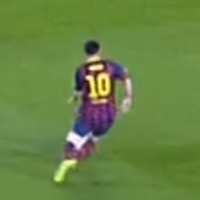
\includegraphics[width=.4\linewidth]{./images/resize_barcelona2.png}
        \captionof{figure}{En la imagen se observa la falta de resolución. Los
        bordes se ven difusos.}
        \label{fig:barsa3}
    \end{minipage}%
    \begin{minipage}[t]{.5\textwidth}
        \centering
        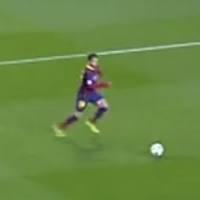
\includegraphics[width=.4\linewidth]{./images/resize_barcelona3.png}
        \captionof{figure}{La imagen muestra varias de las dificultades del
          problema: la baja resolución y el
          diminuto tamaño de la pelota con respecto al jugador.  }
        \label{fig:barsa4}
    \end{minipage}
\end{figure}

\subsection{Complejidad del Análisis en Tiempo Real}

Al tener una resolución de \textit{1080p} (aproximadamente dos millones de
pixels por cuadro), el procesamiento de cada pixel debe tomar a lo sumo 20
nanosegundos.  Para lidiar con esta restricción se puede utilizar información
adicional de la que se disponga respecto al video con el objeto de evitar
procesar pixels de poca o nula utilidad para el seguimiento. Un ejemplo de esto
es descartar pixels que estén fuera de la cancha, ya que es probable que la
cámara encuadre más que el campo de juego, abarcando las gradas, el público
espectador, publicidades alrededor del campo de juego, entre otros.

Muchos autores han desarrollado algoritmos automáticos de seguimiento de
objetos en secuencias de imágenes\cite{IFTrace, alp, local-learning, MHT-2}.
Todos ellos están basados en soluciones de ecuaciones diferenciales en
derivadas parciales y resultan aceptablemente robustos, pero tienen severas
restricciones que impiden que se utilicen para aplicaciones en tiempo real.

Nuestra investigación utiliza el algoritmo de contornos
activos\cite{fast-level-set}, el cual no utiliza ecuaciones diferenciales
(haciéndolo apto para aplicaciones en tiempo real) y además hace un análisis
local de los objetos seguidos en la imagen, lo cual hace que el tiempo de
análisis de un cuadro sea dependiente de la resolución de los jugadores e
independiente de la resolución del video.

\subsection{Distorsión de la lente}

Al utilizar una única cámara para captar la cancha entera se corre el riesgo de
tener distorción en los puntos de la imagen más alejados al foco de la cámara.
Este es el llamado ``efecto de ojo de buey'' e introduce mucho error, por ejemplo
en la aplicación de la homografía, por lo
tanto se debe aplicar una corrección. Una lente apropiada y bien calibrada
puede reducir este error, pero nunca puede ser eliminado totalmente. Sólo
puede evitarse utilizando una mejor técnica de filmación.

\subsection{Oclusiones entre jugadores}

En un partido es muy común que ocurran oclusiones entre los jugadores. El
sistema debe poder tolerar la oclusión parcial o total de los jugadores.
Esto puede llevar a situaciones muy difíciles de automatizar. Una situación
difícilmente automatizable sucede cuando dos jugadores del mismo equipo (con
vestimenta muy similar) se encuentren alineados con respecto a la cámara.
Se pueden agregar reglas para intentar que el método no se confunda, cuando
los jugadores se separen, quién es quién, pero no hay una solución evidente.

Por ejemplo, se puede utilizar información de cuadros anteriores para
estimar la velocidad de cada uno y estimar sus nuevas posiciones, pero esto
es poco efectivo si los jugadores cambian de velocidad mientras uno ocluye
al otro, o si la velocidad era muy similar al momento de generarse la oclusión.

Otra situación problemática similar es una jugada de córner, donde las
oclusiones entre varios jugadores son muy numerosas, lo que agrega a la
restricción de tiempo real mayor complejidad, ya que la resolución de
oclusiones debe ser muy eficiente en tiempo.

\section{Contornos Activos}

La segmentación basada en contornos activos se basa en definir una región en base a su contorno.
El contorno o borde de una región $\Omega_i$ se representa por una curva paramétrica dada por:

\begin{equation}
    C_i(s) = (x_i(s), y_i(s))
\end{equation}

donde $0 \leq s \leq S_i$, y $C_i(0) = C_i(S_i)$, siendo $S_i$ el total de puntos que conforman la curva.
Es decir, $C_i$ es una curva cerrada.

Se definen tantos contornos como objetos de interés haya en la secuencia ($i$ es un entero entre 1 y el número de objetos).
Adicionalmente, se considera una región $\Omega_0$ que contiene a todo punto que no forma parte de ninguna otra región.
Se la denomina \textit{región de fondo}.

Se declara una función de probabilidad $p$ que permite saber que tan probable es que un píxel forme parte de una dada región.
Para esto, es necesaria una función $v$ que dado un píxel, devuelve un vector $v(x)$ de caracteristicas, por ejemplo los valores RGB del pixel.
Esto permite calcular $p(v(x) \vert \Omega_i)$, la probabilidad de que un píxel $x$ forme parte de una región $\Omega_i$ .
Estas funciones dependen de la secuencia particular a ser analizada, por lo que varían dependiendo del caso de estudio.
Como ejemplo, se toman los valores RGB como vector de características y
$p(v(x) \vert \Omega_i) = \| v(x) - v_i \| $, donde $v_i$ es el valor promedio RGB de todo pixel en la región $\Omega_i$.

Se define la función de energía de los contornos:

\begin{equation}
    \label{eq:ac-energy}
    E = - \sum_{m=0}^{M}{\int_{\Omega_m}{\log{p(v(x) \vert \Omega_m)} dx} + \lambda \int_{C_m}{ds}}
\end{equation}

Los algoritmos basados en contornos activos, buscan minimizar esta ecuación. Si el valor de $E$ es mínimo para un cuadro, se
debería haber encontrado la mejor aproximación de la región de los objetos interés. De \ref{eq:ac-energy} se
deriva la ecuación de evolución de cualquier curva $C_m$:

\begin{eqnarray}
    \frac{dC_m}{dt} &=& (F_d + F_s) \overrightarrow{N}_{C_m} \\
    F_d &=& \log{p(v(x) \vert \Omega_m) / p(v(x) \vert \Omega_0)} \\
    F_s &=& \lambda \kappa_m \label{eq:ac-formal}
\end{eqnarray}

$F_d$ y $F_s$ son fuerzas derivadas de la ecuación de energía. $F_d$ representa la competencia entre regiones y $F_s$ un
suavizado. $\kappa_m$ es la curvatura de la curva $C_m$.

Existe otra formulación del problema de evolución de curvas, que consiste en
representar la curva como el nivel cero de una superficie $\phi$ (ver \cite{Osher88}).

\section{Implementación Numérica}

Se toma de referencia la implementación segun \citeauthor{fast-level-set} (ver \cite{fast-level-set}).
En la implementación, el borde de un contorno $C_m$ se representa usando dos conjuntos de píxeles
correspondientes a los bordes interno y externo, $L_{in}$ y $L_{out}$
respectivamente. Entonces, la evolución se realiza intercambiando píxeles entre
estos dos conjuntos.

A continuación se detalla la técnica para la segmentación de un solo objeto de
interés que se puede fácilmente extrapolar y utilizar para la
segmentación de múltiples objetos
\footnote{Para la segmentación de múltiples objetos basta con marcar las distintas regiones con un identificador
distinto y seguirlas por separado.}.

El objeto de interés $\Omega_{1}$ y el fondo $\Omega_{0}$ cumplen
$\Omega_{1}\cup\Omega_{0} = I_{k}$ donde $I_{k}$ es la imagen del cuadro $k$ de
la secuencia de imágenes, y $\Omega_{1}\cap\Omega_{0} = \emptyset$. Cada una de
las regiones está caracterizada por su vector característico $v_{m}, m =
\{0,1\}$.

Se define una función $\phi(x)$ que indica si un píxel $x$ pertenece a una región o al fondo de la siguiente manera:

\begin{equation}
\phi(x) =
\left\{
    \begin{array}{ll}
        3  & \mbox{si } x \in \Omega_{0} \mbox{  y  } x \notin L_{out} \\
        1  & \mbox{si } x \in L_{out}\\
        -1  & \mbox{si } x \in L_{in}\\
        -3 & \mbox{si } x \in \Omega_{1} \mbox{  y  } x \notin L_{in} \\
    \end{array}
\right.
\end{equation}

Los conjuntos $L_{in}$ y $L_{out}$ se definen como

\begin{equation}
    L_{in} = \{ x \mbox{ es un píxel } \vert \mbox{    }  \phi(x) < 0 \mbox{ y } \exists y \in N_{4}(x) \mbox{ de modo que } \phi(y) > 0 \}
\end{equation}

\begin{equation}
    L_{out} = \{ x \mbox{ es un píxel } \vert \mbox{    } \phi(x) > 0 \mbox{ y } \exists y \in N_{4}(x) \mbox{ de modo que } \phi(y) < 0 \}
\end{equation}

donde $N_{4}(x) = \{ y \mbox{ es un pixel } \vert \mbox{   } |x-y| = 1 \}$, son los píxeles
vecinos del píxel $x$.

El algoritmo de segmentación es un algoritmo de dos ciclos, ya que luego de la
especificación inicial de la curva en forma supervisada \footnote{Podría no ser
supervisada. Existen variantes con determinaciones semi-supervisadas del objeto
de interés, así como también detección automática basada en ciertas
características predefinidas.} se intercambian los píxeles de $L_{in}$ y
$L_{out}$ en dos ciclos. En el primero, se aplica la fuerza $F_{d}(x)$, y en el
segundo se aplica $F_{s}(x)$ para la regularización.

En el primer ciclo, se ejecutan los siguientes pasos $N_{a}$ veces, donde $ 0 <
N_{a} < max(filas, columnas)$.

\begin{enumerate}

    \item Para cada $x \in L_{out}$, si $F_{d}(x) > 0$ entonces borrar $x$ de $L_{out}$ y agregarlo a $L_{in}$. \\
    Luego, $\forall y \in N_{4}(x)$, con $\phi(y) = 3$, agregar $y$ to $L_{out}$ y hacer $\phi(y) = 1$.

    \item Después del paso 1 algunos de los píxeles $x$ en $L_{in}$ pasan a ser píxeles internos. \\
    Por lo tanto, se sacan de $L_{in}$ y se hace $\phi(x) = -3$.

    \item Para cada $x \in L_{in}$ , si $F_{d}(x) < 0$ entonces, borrar $x$ de $L_{in}$ y agregarlo a $L_{out}$. \\
    Luego, $\forall y \in N_{4}(x)$, con $\phi(y) = -3$, agregar $y$ a $L_{in}$ y hacer $\phi(y) = -1$.


    \item Después del paso 3 algunos de los píxeles $x$ en $L_{out}$ pasan a ser píxeles externos. \\
    Por lo tanto, se sacan de $L_{out}$ y se hace $\phi(x) = 3$.

\end{enumerate}

En el segundo ciclo, la curva se suaviza utilizando un filtro Gaussiano, de tal
forma que la fuerza de evolución es $F_{s}(x) = G \otimes \phi(x)$. Para aplicar $F_s$ se usan los mismos
pasos que para $F_d$. El resultado final es análogo a modificar la curva de acuerdo
a la definición formal dada anteriormente (Ecuación \ref{eq:ac-formal}).

En cada cuadro, el borde del contorno del objeto es actualizado de acuerdo al
resultado obtenido por el algoritmo en el cuadro anterior. En el caso de la
primera imagen, se puede dar de forma supervisada o semi-supervisada por el
usuario, o bien puede ser obtenida de forma automática mediante algoritmos de
aprendizaje complejos basados en características predefinidas.

El algoritmo termina cuando se alcanza la condición de corte, dada por las
ecuaciones \ref{eq:active-contours-stoppingCondition} o cuando se alcanza el numero de iteraciones $N_a$

\begin{equation}
\label{eq:active-contours-stoppingCondition}
    \begin{array}{ll}
        F_{d}(x) \leq 0 & \forall x \in L_{out}\\
        F_{d}(x) \leq 0 & \forall x \in L_{in}
    \end{array}
\end{equation}

%% TODO revisar esto. Movi la sección de COntornos Activos del estado del arte acá arriba pero no se
%% si queda bien así como está. Esta section antes era subsubsection, y la deje abajo de
%% la subsección de contornos activos porque habla de particularidades del algoritmo de contornos activos
%% y me pareció que no daba ponerlo antes de describir y detallar contornos activos. De todas formas
%% hay que chequear la distribución en sections y subsubsections para que tenga una secuencia logica
%% que creo que ahora no la tiene :s.

\section{Algoritmo utilizado}

El correcto funcionamiento del algoritmo de contornos
activos\cite{fast-level-set} depende de una buena selección de la función
característica, para poder distinguir claramente a un jugador respecto a otros
objetos o respecto del fondo. En casos como el ilustrado por la figura
\ref{fig:camiseta}, elegir una función característica resulta sencillo, ya que
con elegir el color de la camiseta se asegura una buena descripción del contorno
a seguir. Sin embargo, la imagen de la figura \ref{fig:camiseta-rayada} introduce
uno de los problemas en la selección de la función característica. Se puede ver que
las diferencias entre ambos colores del objeto hacen dificil identificarlos a ambos
con una misma caracteristica.

%TODO meter alguna referencia?
%TODO que onda las otras imagenes?
\begin{figure}[H]
    \centering
    \begin{minipage}[t]{.5\textwidth}
        \centering
        
\includegraphics[width=.4\linewidth]{./images/rect2995.png}
        \captionof{figure}{Camiseta de color lisa. El color de la camiseta es claramente distinguible del fondo.}
        \label{fig:camiseta}
    \end{minipage}%
    \begin{minipage}[t]{.5\textwidth}
        \centering
        
\includegraphics[width=.4\linewidth]{./images/rect2996.png}
        \captionof{figure}{Camiseta de 2 colores rayada. Las franjas de la camiseta son claramente distinguibles entre sí y el fondo.}
        \label{fig:camiseta-rayada}
    \end{minipage}
\end{figure}

Este es un desafío grande debido principalmente a dos problemas:
\begin{itemize}

\item Selección de colores: si la cancha tiene un color muy similar a la
  camiseta de un equipo, ¿cómo será posible distinguirlos? Se exploran
  distintas alternativas, como utilizar otra codificación de color.

\item Textura de los jugadores: esto representa un gran problema por varias
  razones. La primera es que la técnica de contornos activos está atada a la
  selección de una o varias características del objeto a seguir. Como la
  característica más distintiva es el color, la técnica se basá en ella. Pero
  para camisetas con más de un color, se vuelve absurda la idea de encontrar
  un color característico, dado que no existe.  Esta dificultad se ilustra en
  la imágenes de las figuras \ref{fig:barsa1} y \ref{fig:barsa2}. Por
  otro lado, dada la escasa cantidad de pixels que representan a un jugador,
  debido a nuestro enfoque de única cámara, cualquier tipo de análisis se torna
  complejo cuando sus características no están lo suficientemente definidas
  como para diferenciarlas (ya sea de otros jugadores o del fondo).

\end{itemize}

\begin{figure}[H]
    \centering
    \begin{minipage}{.5\textwidth}
        \centering
        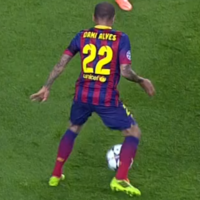
\includegraphics[width=.4\linewidth]{./images/resize_barcelona1.png}
        \captionof{figure}{Desde este punto de vista, se puede observar al menos 3 fuertes
        características (colores) en la camiseta del jugador, rojo, azul y amarillo.}
        \label{fig:barsa1}
    \end{minipage}%
    \begin{minipage}{.5\textwidth}
        \centering
        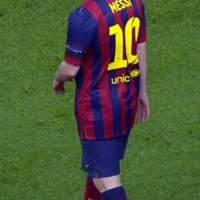
\includegraphics[width=.4\linewidth]{./images/resize_barcelona4.png}
        \captionof{figure}{Incluso con mayor resolución, las distintas características (como ser los colores azul, amarillo, y rojo) dificultan el seguimiento con contornos activos.}
        \label{fig:barsa2}
    \end{minipage}
\end{figure}

%TODO aca mepa que pueden ir varias imagenes.
% 1 de un tracking de de un jugador de remera blanca (podría ser PRE y POST, osea sin pintar y pintado)
% 1 de un tracking de un jugador de boca (again PRE y POST)
% 1 de la pelota? Para mostrar la cantidad infima de pixels?



\section{Solución propuesta}
\label{sec:solution}

En esta sección describimos las distintas tecnicas aplicadas. Primero describimos algoritmos para
ignorar los elementos del fondo de la imagen en \ref{sec:background-elimination}. Luego, explicamos
como utilizamos el algoritmo contornos activos\cite{fast-level-set} y las modificaciónes necesarias
en \ref{sec:ac}. Finalmente, detallamos la integración final entre las distintas tecnicas, que es
la que analizamos en la siguiente seccion \ref{sec:results}.

\subsection{Eliminación de fondo por varios métodos}
\label{sec:background-elimination}
Problemas y soluciones (tal vez como subsubsection)

\subsubsection{Tribuna y publicidades}
% Simplemente como ponemos en negro para que no interfiera

\subsubsection{Energia}
  * Método de la energía

\subsubsection{Eliminación de lineas}
  * Eliminación de lineas por Detector de borde + umbral + morfología

\subsubsection{Eliminación del pasto}
  * Eliminación de colores de cancha por histograma de colores


\subsection{Contornos activos}
\label{sec:ac}

- Características

  * Colores del jugador
  * Aprendizaje
  * Múltiples características
  * Selección de máximos en histograma con bfs

- Descriptores

\subsection{Algoritmo final}
\label{sec:alg-final}
% Que onda esta seccion? Me parece medio tirada de los pelos la idea

- Eliminación de lineas por detector de borde + umbral + morfología
- Múltiples características
- Descriptores
- Imágenes de cómo resolvemos algunos casos extremos

- Opcional para equipos difíciles de detectar: seguimiento por complemento
  - eliminación de colores de cancha por histograma + ronda de contornos

- Que lastima que no tuvimos trackeo de pelota porque hubiese dado mejores datos


\chapter{Resultados}
\label{chap-results}

% TODO: Discutir sobre diferencias semanticas entre algoritmo, implementación, programa... etc. Qué usamos y que cosas las tomamos como sinonimos. Tal vez hacer un glosario...
Esta sección presenta un análisis de los resultados obtenidos de la ejecución
del algoritmo sobre distintos videos. % [Llenar más]

Se presentan las salidas de la implementación, métricas utilizadas para evaluar la performance del algoritmo. A lo largo del capítulo se discuten alternativas propuestas y descartadas, resultados parciales, y otras métricas que no se calcularon.

\section{Aplicación}

La aplicación implementada incorpora una interfaz gráfica utilizada tanto para dar instrucciones como para recibir información acerca del partido y del funcionamiento del algoritmo. La misma cuenta con una interfaz donde se muestra a los jugadores, una lista de jugadores siendo seguidos, un mapa de calor de espacios ocupados por los jugadores, y una imágen que permite al operador evaluar el correcto funcionamiento del algoritmo.

Para comenzar la ejecución, el algoritmo requiere que el operador identifique la posición de los jugadores en la imagen inicial de la secuencia. % [ TODO: Completar con chamuyo ]

Un paso adicional es el de determinar puntos a utilizar para el cálculo de la homografía. Los datos necesarios son al menos cuatro parejas de puntos. De estas parejas, el primer punto es una coordenada la imagen en perspectiva y el otro punto es la coordenada
en un plano bidimensional. Con cuatro de estas relaciones, se puede calcular la matriz que resuelve la homografía para cualquier otro punto. % [ TODO: esto no queda claro ]

Una vez que el programa tiene estos datos, el algoritmo de contornos activos puede comenzar a correr. Existen dos modos, uno que avanza sólo ante la indicación del operador (mecánica ``cuadro por cuadro'') y otro modo que avanza automáticamente cada vez que se computa un cuadro (mecánica ``tiempo real''). % [ TODO: algo de amor a este párrafo ]

Cada cuadro, una ventana muestra las posiciones actualizadas de los jugadores. El usuario puede seleccionar un jugador en particular y ver en detalle información sobre su posición, velocidad promedio, actual, y máxima desde el comienzo del seguimiento, y un mapa de calor que muestra con colores próximos al rojo los lugares más visitados por el jugador. Además, en un archivo se escribe la posición de cada jugador por cada frame.

De manera opcional, en cada cuadro se guarda en disco duro una copia del estado actual del seguimiento para referencia futura.

\section{Material utilizado}

Se utilizaron principalmente dos videos, uno correspondiente a un partido entre los equipos argentinos de los clubes Boca Juniors e Independiente; y un segundo video en el cual se enfrentan los equipos Independiente y San Lorenzo. Se detalla a continuación las características de las imágenes extraídas de esos videos.

\begin{itemize}
  \item \textbf{Boca vs Independiente:}
  \item \textbf{Independiente vs San Lorenzo:}
\end{itemize}

Además, se tomaron pequeños cortes de tres videos de fútbol televisado en los cuales la cámara se encuentra relativamente estática y se analizó la correctitud del seguimiento en estos casos, contando con mayor resolución pero sin poder efectuar exitosamente la eliminación de fondo o la correlación a un plano bidimencional por homografía % [ TODO: ESTO ESTÁ ESCRITO CON LA ** ]

\begin{itemize}
  \item \textbf{Manchester City vs Barcelona:}
  \item \textbf{Real Madrid vs Borussia Dortmound:}
  \item \textbf{Argentina vs Suiza:}
\end{itemize}

\section{Evaluación del método}

Se evaluó cualitativamente por un operador que los contornos de los jugadores según el algoritmo modificado de contornos activos no correspondían a los jugadores, como es el caso de trabajos citados en el estado del arte (ver \cite{papers-tanos}). Se atribuye esto a la baja calidad de los videos que se pudieron obtener, y la poca capacidad de procesamiento en comparación. (TODO: Completar esto justificando mejor).

Dado esto, se procedió a evaluar cuántas veces sucedía esta discrepancia por unidad de tiempo. Esta métrica, resumida como la cantidad de errores del algoritmo por cada cien cuadros, se intentó minimizar durante el estudio de las variantes de la aplicación.

Otra métrica que se buscó minimizar es el tiempo de demora por cuadro procesado, hasta intentar alcanzar una velocidad de $24$ cuadros por segundo (equivalente a $42$ milisegundos por cuadro), la velocidad de los videos utilizados.


% TODO chequear la forma de referirse a NUESTRO algoritmo sin decir la palabra NUESTRO :s
%% TODO: Ojo, a partir de acá hablamos en pasado. Deberíamos ser consistentes,
%% por como arrancamos en el resuemen, la intro y por lo que dice la mina
%% deberiamos usar el presente o eso de "se plantea, se define, etc..."

\section{Comparación con IFTrace}
\label{sec:iftrace}

El algoritmo de seguimiento IFTrace, propuesto por \citeauthor*{IFTrace}, es un
algoritmo robusto que soporta cambios de iluminación y forma, oclusiones y se
centra en hallar características representativas de la textura de los objetos a
seguir. Es capaz de recuperarse de errores menores y permite el seguimiento de
múltiples objetos a la vez.

Un algoritmo de este tipo podría proporcionar una solución al problema. Para
comprobarlo, se llevaron a cabo algunas pruebas utilizando un video sintético
creado para este fin, y un video real de un partido de fútbol. En las Figuras
\ref{fig:sample-happy-occluded} y \ref{fig:sample-boca} pueden observarse los
primeros cuadros de cada video. Pueden apreciarse a simple vista las marcadas
diferencias entre ambos videos, como por ejemplo la resolución de la imagen y
el tamaño y la complejidad de los objetos de inteŕes.

\begin{figure}[H]
    \centering
    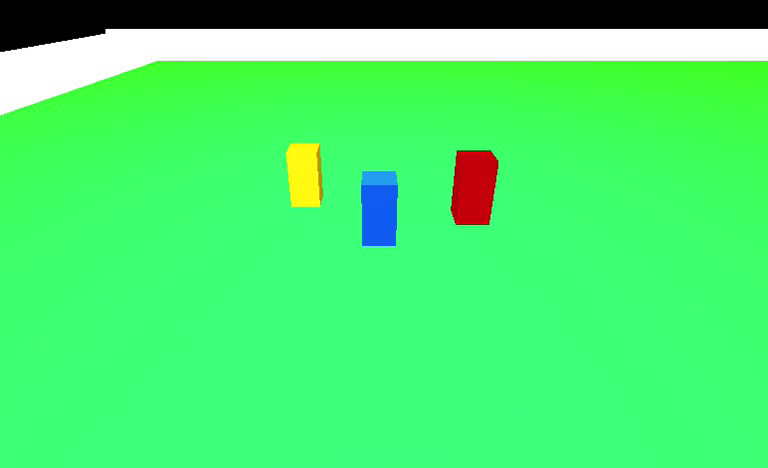
\includegraphics[width=\linewidth]{./images/sample_happy_occluded.png}
    \caption{Muestra de un cuadro del video sintético de prueba.}
    \label{fig:sample-happy-occluded}
\end{figure}

\begin{figure}[H]
    \centering
    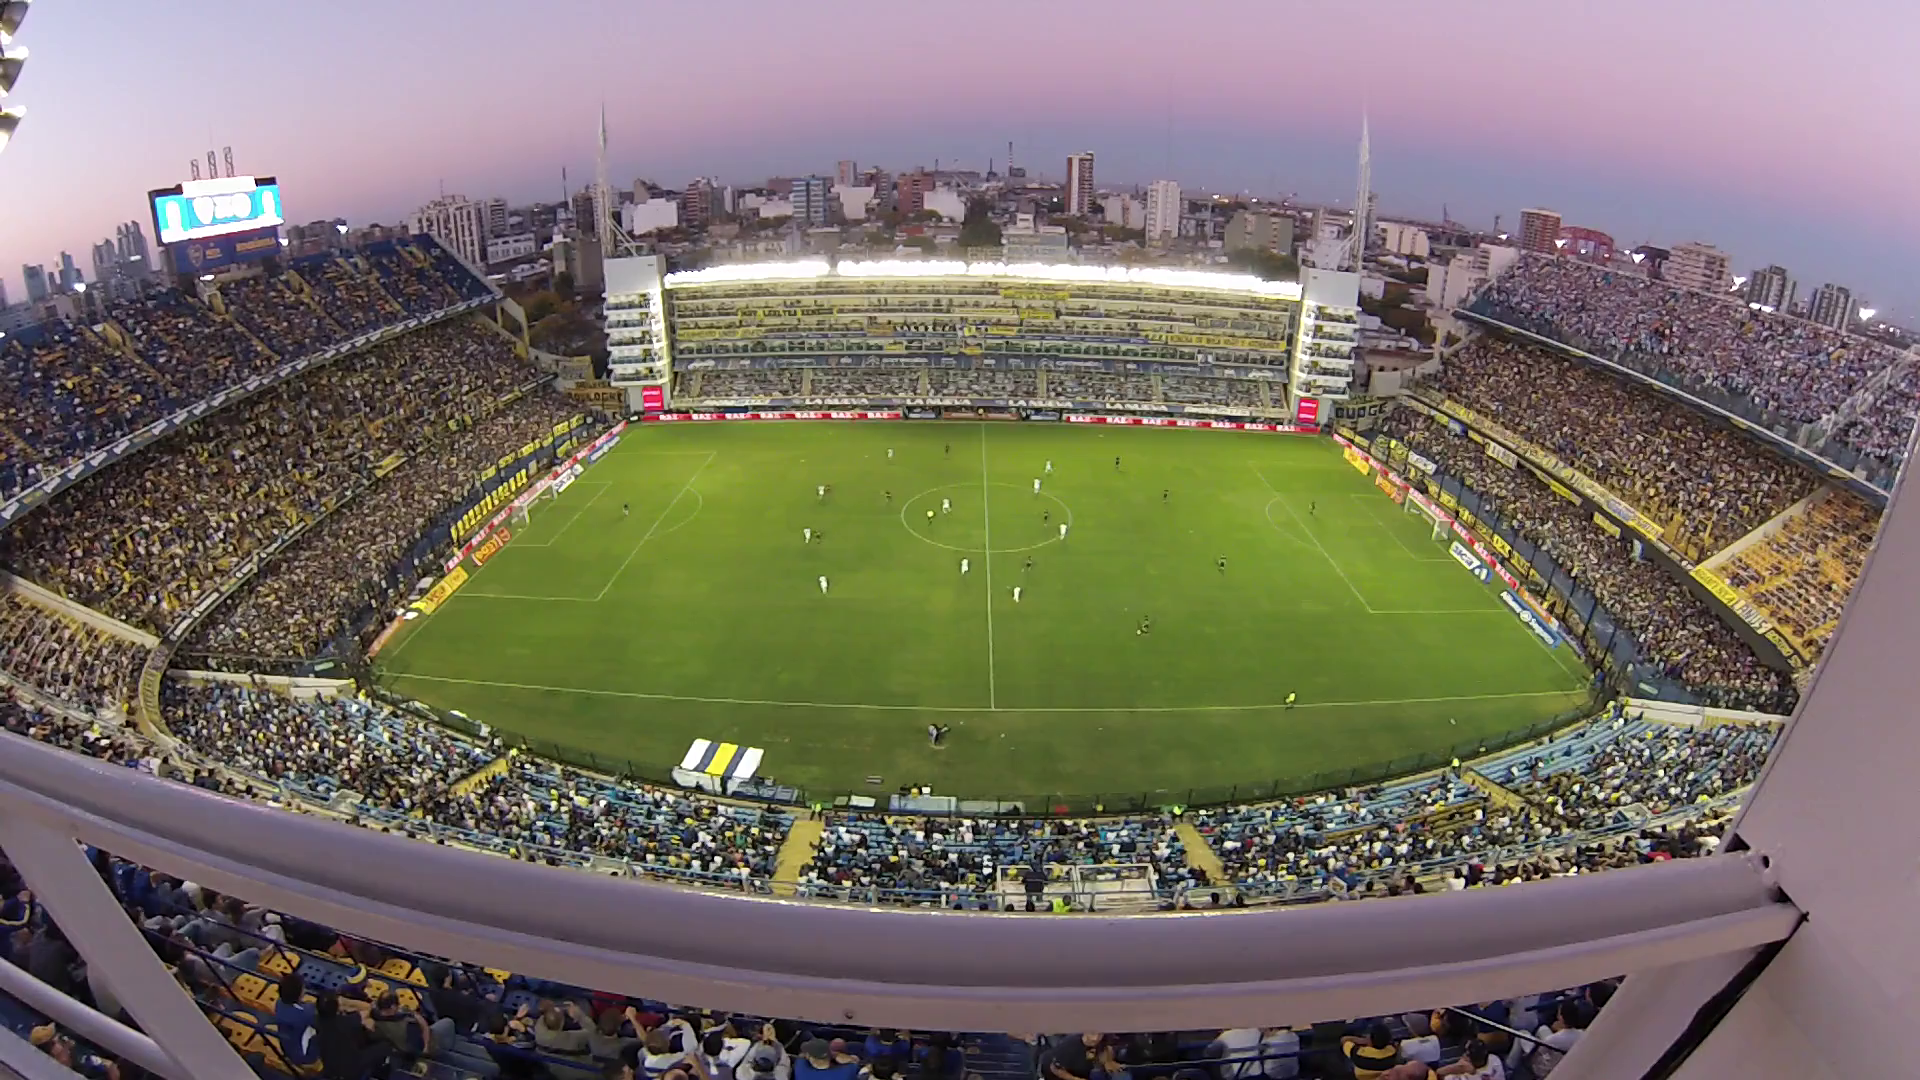
\includegraphics[width=\linewidth]{./images/sample_boca.png}
    \caption{Muestra de un cuadro del video real de un partido de fútbol.}
    \label{fig:sample-boca}
\end{figure}

Como se puede ver en la Figura \ref{fig:happy-occluded-iftrace}, IFTrace logra
un correcto seguimiento de múltiples objetos en el video sintético.  También
puede observarse, en la Figura \ref{fig:boca-iftrace}, como sigue correctamente
a un jugador en el video real.  Sin embargo, el seguimiento sólo es exitoso
durante unos pocos cuadros, ya que, en el cuadro 17, el algoritmo cae en un
error del cual sólo una corrección manual puede sacarlo. Este tipo de correción
semi-supervisada no está contemplada en el algoritmo de IFTrace.

\begin{figure}[H]
    \centering
    \begin{tabular}{cccc}
        \subfloat[Cuadro 1]{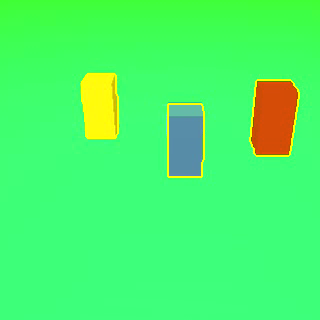
\includegraphics[width = 1.5in]{./images/cropped_happy_occluded_00001.png}} &
        \subfloat[Cuadro 5]{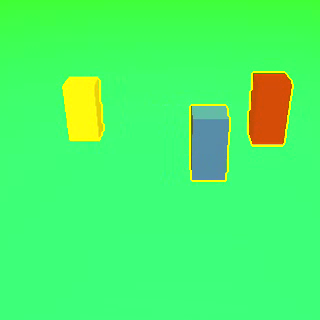
\includegraphics[width = 1.5in]{./images/cropped_happy_occluded_00005.png}} &
        \subfloat[Cuadro 8]{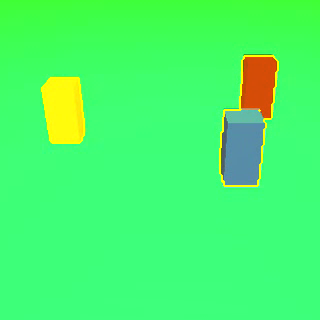
\includegraphics[width = 1.5in]{./images/cropped_happy_occluded_00008.png}} &
        \subfloat[Cuadro 12]{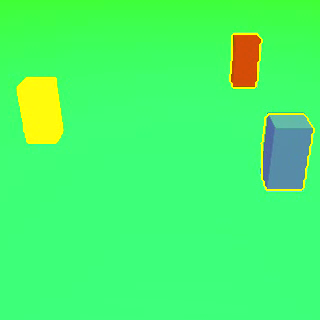
\includegraphics[width = 1.5in]{./images/cropped_happy_occluded_00012.png}}
    \end{tabular}
    %% NASTY hack to make refernce work with figures and subfigures, put \label inside \caption env, little bird told me
    \caption{IFTrace funcionando en una secuencia de cuadros de video sintético.
    \label{fig:happy-occluded-iftrace}
    }
\end{figure}

\begin{figure}[H]
    \centering
    \begin{tabular}{cccc}
        \subfloat[Cuadro 9]{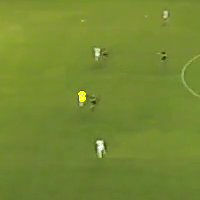
\includegraphics[width = 1.5in]{./images/cropped_boca_00009.png}} &
        \subfloat[Cuadro 12]{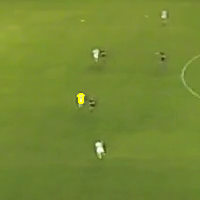
\includegraphics[width = 1.5in]{./images/cropped_boca_00012.png}} &
        \subfloat[Cuadro 14]{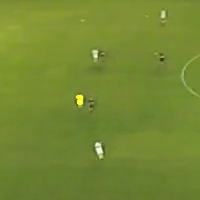
\includegraphics[width = 1.5in]{./images/cropped_boca_00014.png}} &
        \subfloat[Cuadro 17]{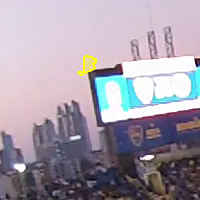
\includegraphics[width = 1.5in]{./images/cropped_boca_00017.png}}
    \end{tabular}
    %% NASTY hack to make refernce work with figures and subfigures, put \label inside \caption env, little bird told me
    \caption{Seguimiento de un jugador en un video real utilizando IFTrace.
    \label{fig:boca-iftrace}
    }
\end{figure}

\begin{figure}[H]
    \centering
    \begin{tabular}{cccc}
        \subfloat[Cuadro 1]{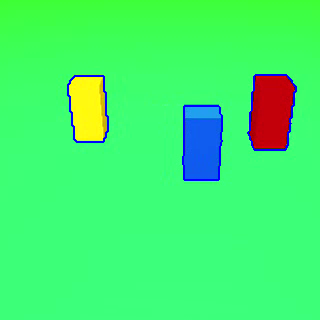
\includegraphics[width = 1.5in]{./images/cropped_processing2.png}} &
        \subfloat[Cuadro 5]{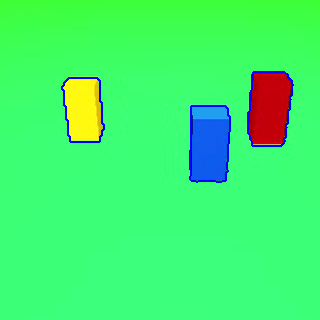
\includegraphics[width = 1.5in]{./images/cropped_processing5.png}} &
        \subfloat[Cuadro 8]{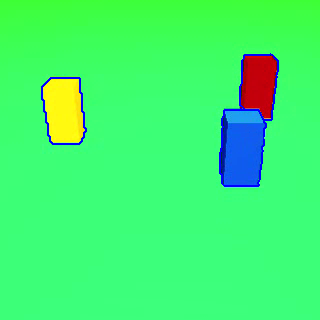
\includegraphics[width = 1.5in]{./images/cropped_processing14.png}} &
        \subfloat[Cuadro 12]{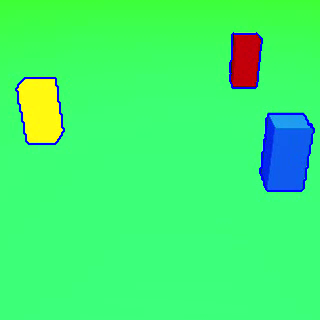
\includegraphics[width = 1.5in]{./images/cropped_processing25.png}}
    \end{tabular}
    %% NASTY hack to make refernce work with figures and subfigures, put \label inside \caption env, little bird told me
    \caption{Nuestro algoritmo en funcionamiento en un video sintético.
    \label{fig:happy-occluded-activeContour}
    }
\end{figure}

\begin{figure}[H]
    \centering
    \begin{tabular}{cccc}
        \subfloat[Cuadro 2]{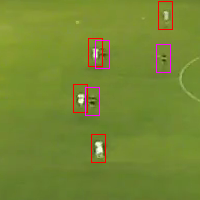
\includegraphics[width = 1.5in]{./images/cropped_rendered002.png}} &
        \subfloat[Cuadro 12]{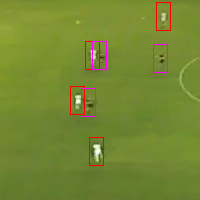
\includegraphics[width = 1.5in]{./images/cropped_rendered007.png}} &
        \subfloat[Cuadro 14]{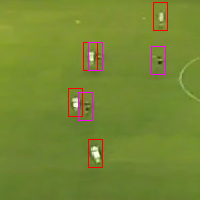
\includegraphics[width = 1.5in]{./images/cropped_rendered012.png}} &
        \subfloat[Cuadro 17]{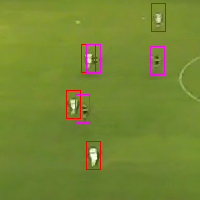
\includegraphics[width = 1.5in]{./images/cropped_rendered017.png}}
    \end{tabular}
    %% NASTY hack to make refernce work with figures and subfigures, put \label inside \caption env, little bird told me
    \caption{Seguimiento de los jugadores en un video real mediante el algoritmo de contornos activos modificados.
    \label{fig:boca-activeContour}
    }
\end{figure}

Como se puede observar en la Figura \ref{fig:happy-occluded-activeContour},
el algoritmo de contornos activos modificado logra seguir con éxito a los
objetos de interés en el video sintético. Además, también se obtiene un
resultado positivo en el video real en la situación en que IFTrace pierde al
jugador, como puede observarse en la Figura \ref{fig:boca-activeContour}.

\subsection{Evaluación de comportamiento}

Otro punto importante de comparación entre los dos algoritmos es su tiempo de
ejecución, es decir el tiempo que tarda en llevar a cabo su trabajo.  De
acuerdo a las mediciones realizadas con un video real de un partido de fútbol,
siguiendo a un solo jugador, el tiempo promedio que tarda IFTrace por cuadro es
6.962 segundos, mientras que nuestro algoritmo tiene un tiempo promedio de
0.712 segundos. Se puede observar que se encuentra un orden magnitud por debajo
de IFTrace.
%% 6.9628571428571435 si quieren los decimales
%% TODO verificar nuestro numero!!!

Cabe destacar que ambos algoritmos podrían verse beneficiados de ciertas
optimizaciones, como ser por ejemplo la programación en GPU y la reducción de
operaciones de \textit{Input/Output} al almacenamiento secundario (disco duro).

% TODO Esto creo que probablemente terminemos sacandolo right? Que métrica podemos meter?!?!
% - Comparación de nuestros resultados vs los de ellos (Métrica: cantidad de jugadores perdidos por frame -- o si se nos ocurre una mejor ambas o esa)


\chapter{Conclusiones}
\label{chap-conclusion}

- Mal material, imposible agarrar la pelota y difícil los jugadores
- Resultados aceptables


\printbibliography

\begin{comment}

- Algoritmo de deteccion de fondo: cosas que no son la cancha en el video arruinan las mediciones
  => Poner en negro toda parte del video que no sea la cancha

- Funcion de feature de contornos activos
  + Tomar promedio de color del contorno inicial no soporta camisetas rayadas
  + Tampoco aguanta camisetas con mucha iluminacion
  => Busqueda de nuevos features
    - sigma
    - coeficiente de variacion: ???
    - distintos color-spaces: algunos color spaces funcionan mejor para un tipo de camiseta que otro. seria necesario tener varios features distintos y saber seleccionar el mejor

- Distorcion de la lente introduce error en la homografia
  => Algoritmos de correcion de la lente
     - El factor de correcion es distinto para cada video
     - Es dificil de calcular programaticamente

- Jugadores distantes se borronean mucho
  => ???

- La pelota es muy chica
  => ???

- Cuando un jugador marca a otro, suele recorrer mucha distancia oculto o semi oculto
  => ???

- Además de distorción de la lente, la RESOLUCION: al agarrar TODA la cancha en una toma los jugadores MUY chicos, y la pelota más
    => ???

- Las canchas tienen diferentes medidas (varían en un cierto rango). Esto afecta a la homografía
    => Adaptar la homografía a las dimensiones de cada cancha.

- Como relacionar posiciones relativas de los jugadores teniendo una vista 3D con perspectiva
    => Homografía
    (Muy básico?)

\end{comment}

\end{document}
